\documentclass[12pt,twoside,openright]{report}

% Hyperlink references
\usepackage[pdfborder={0 0 0}]{hyperref}
% PGF diagrams
\usepackage{pgf}
\usepackage[utf8]{inputenc}\DeclareUnicodeCharacter{2212}{-}
% Page margins
\usepackage[margin=25mm]{geometry}
% Subfigures
\usepackage{caption}
\usepackage{subcaption}
% Bibliography
\usepackage[style=numeric-comp,sorting=none]{biblatex}
% Images
\usepackage{graphicx}
% Directory tree diagram
\usepackage{dirtree}
% Simple tree diagrams
\usepackage[linguistics]{forest}
\usepackage{adjustbox}
% Algorithms
\usepackage[ruled]{algorithm2e}
% Verbatim++
\usepackage{alltt}
% Text colour
\usepackage{xcolor}
% Better verbatim
\usepackage{fancyvrb}
% TikZ diagrams
\usepackage{tikz}
% UK date
\usepackage[UKenglish]{babel}
\usepackage{csquotes}
% Paragraph spacing
\usepackage{parskip}


\addbibresource{bibliography.bib}

%\renewcommand{\baselinestretch}{1.1}
\raggedbottom

\DeclareRobustCommand{\setmetre}[2]{\ensuremath{
  \vcenter{\offinterlineskip
    \halign{\hfil##\hfil\cr
            $\scriptstyle#1$\cr
            \noalign{\vskip1pt}
            $\scriptstyle#2$\cr}
  }}
}

\definecolor{SPpink}{RGB}{255,20,147}
\definecolor{SPblue}{RGB}{30,144,255}
\definecolor{SPorange}{RGB}{255,140,0}
\definecolor{SPgreen}{RGB}{97,206,60}

\begin{document}

%%%%%%%%%%%%%%%%%%%%%%%%%%%%%%%%%%%%%%%%%%%%%%%%%%%%%%%%%%%%%%%%%%%%%%%%
% Title

\begin{titlepage}
    \pagestyle{empty}

    \rightline{\LARGE \textbf{Max Johnson}}

    \vspace*{60mm}
    \begin{center}
    \Huge
    \textbf{Musical micro-timing for live coding} \\[5mm]
    Computer Science Tripos -- Part II \\[5mm]
    Clare College \\[5mm]
    \today
    \end{center}
\end{titlepage}

%%%%%%%%%%%%%%%%%%%%%%%%%%%%%%%%%%%%%%%%%%%%%%%%%%%%%%%%%%%%%%%%%%%%%%%%
% Proforma, table of contents and list of figures

\pagestyle{plain}

\section*{Declaration}

I, [Name] of [College], being a candidate for Part II of the Computer Science Tripos, hereby declare that this dissertation and the work described in it are my own work, unaided except as may be specified below, and that the dissertation does not contain material that has already been used to any substantial extent for a comparable purpose. I am content for my dissertation to be made available to the students and staff of the University.

\bigskip
\leftline{Signed [signature]}

\medskip
\leftline{Date [date]}


\newpage
\chapter*{Proforma}

{\large
\begin{tabular}{ll}
Name:               & \bf Max Johnson                       \\
College:            & \bf Clare College                     \\
Project Title:      & \bf Musical micro-timing for live coding \\
Examination:        & \bf Computer Science Tripos -- Part II, July 2022  \\
Word Count:         & \bf N/A \\
Project Originator: & Mark Gotham                    \\
Supervisor:         & Mark Gotham                    \\ 
\end{tabular}
}


\section*{Original aims of the project}

TBC


\section*{Work completed}

TBC

\section*{Special difficulties}

TBC
 
\newpage
\tableofcontents

%%%%%%%%%%%%%%%%%%%%%%%%%%%%%%%%%%%%%%%%%%%%%%%%%%%%%%%%%%%%%%%%%%%%%%%

\pagestyle{headings}

\chapter{Introduction}

Text.



\chapter{Preparation}

This chapter will introduce the core theories and background material necessary
to understand the project. I will explain some key concepts in music theory and
live coding and give an overview of the case study musical styles. Next, I will
describe the starting point of this project, expand upon the requirements from
the project proposal, and conclude with an outline of the software engineering
techniques used throughout.



\section{Background} \label{background}


\subsection{Musical metre} \label{metre_background}

A beat is a regularly occurring pulse in music. This is usually the pulse you
might tap your foot along to when listening to a piece of music. Musical metre
describes the ways in which beats are grouped and divided within recurring
cycles. This forms different metrical levels within a hierarchy. Division levels
are ones where the beat has been divided into more, shorter durations. Multiple
levels are ones where the beats are grouped into fewer, longer durations. Figure~\ref{fig:metre_hierarchy_example} 
shows the beat level, and some of the division and multiple levels for a simple \ \setmetre{4}{4} time signature, as well as a tree representation of the metrical hierarchy.
A metre is `simple' if its first division level splits the beat into two, and
`compound' if it splits into three \cite{omt2021}.

\begin{figure}
    \centering
    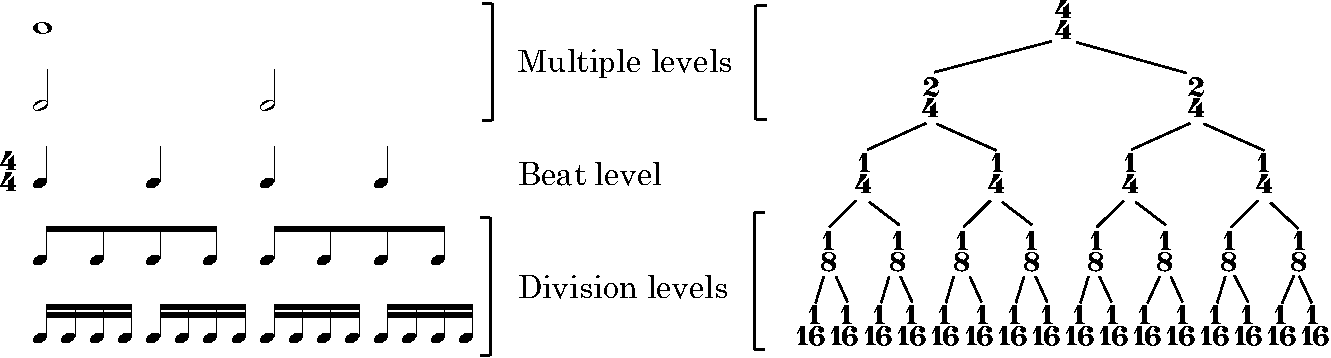
\includegraphics[width=\linewidth]{figures/metre_example.pdf}
    \caption{Example metrical hierarchy for the \setmetre{4}{4} time signature. Left shows the hierarchy as notes in traditional Western music notation. Right shows the hierarchy as a tree of durations.}
    \label{fig:metre_hierarchy_example}
\end{figure}

Every note in a piece of music occurs at a particular metrical position, but
music performed by humans often deviates from these mechanically even timings
\cite{london2012}. The ways in which these deviations occur contribute significantly
to what we call musical style by producing micro-timing effects. Different
musical styles have different micro-timing strategies. A common example is the
long-short pattern in swing rhythms, where every second eighth note (the first
division level) is slightly delayed. This timing information is typically lost
in music notation \textcolor{red}{(see FIGURE for an example of this)}, so musicians have to use
their knowledge and experience of the style to inform their performance of the
micro-timing. This is formalised in Justin London's Many Meters Hypothesis
\cite{london2012}. A metre without any micro-timing is said to be `isochronous',
which means the metric events at each level are equally spaced in time.


\subsection{Live coding} \label{live_coding_background}

Music live coding is a way of creating and performing music by writing and
modifying code in real time. The performer typically projects their code onto a
screen for an audience to follow along with \cite{magnusson2011}. The liveness of the
performance is important -- it is argued that the musician must directly
interact with the running algorithms for it to be truly considered live coding
\cite{collins2011}. Otherwise, there is little difference between this and playing a
recording of synthesised music.

Sonic Pi is a popular live coding language and IDE created by Sam Aaron, which
was designed as an educational tool for teaching programming in schools. It
implements its own domain-specific language written in Ruby, using the
SuperCollider sound synthesis server to produce sounds \cite{aaron2013}. A simple
Sonic Pi program might look like the following:

\begin{BVerbatim}[commandchars=\\\{\}]
play \textcolor{SPpink}{:C4}
sleep(\textcolor{SPblue}{1})
play \textcolor{SPpink}{:C5}
sleep(\textcolor{SPblue}{0.5})
play \textcolor{SPpink}{:C4}
\end{BVerbatim}

This plays the note C3 on the current synthesiser, sleeps for one beat, plays C4,
sleeps for half a beat, then plays C3 again.

A key component of the Sonic Pi language is the \verb'live_loop', which executes a
block of code in a loop in a new thread. This multi-threading allows multiple
musical parts to be played together. To maintain correct timing in the presence
of multiple threads and long execution time, Sonic Pi uses sophisticated
``virtual time'' functionality behind-the-scenes \cite{aaron2014}.

One drawback of Sonic Pi is that it currently doesn't have a built-in notion of
metre or style-specific micro-timing, which is what this project addresses.


\subsection{Case studies} \label{case_studies}

This project uses two different styles of music as case studies for evaluation,
both of which have well-known micro-timing characteristics. The first is jembe
drum music from Mali, which has highly regular micro-timing, and the second is
Viennese waltz music, which offers a Western comparison.

Jembe ensemble music is a style of music involving a small group of drummers
which originated in West Africa. The primary drum is the eponymous jembe, which
is a goblet-shaped drum played with the bare hands. This is usually accompanied
by the dundun, which is a cylindrical drum played with a stick \cite{polak2010}. In a
traditional jembe trio, there are two jembe players and one dundun player, with
Jembe 1 having a lead role, Jembe 2 playing a simple accompaniment, and Dundun
playing a varying pattern that's characteristic of each piece of music
\cite{jacoby2021}. Different playing techniques produce various kinds of sound
(timbre) on each drum, which gives rise to the melodic qualities of the music
\cite{polak2010}.

Jembe music is an ideal case study for this project because it has a highly
consistent micro-timing strategy \cite{polak2010}; Malian drummers have been shown to
have one of the lowest levels of timing variability between performers in the
world \cite{clayton2020}. Compared with other styles of music, jembe music is
relatively constrained in terms of its pitch, timbre, and number of instruments,
which allows for a clear focus on timing.

The Viennese waltz is a style of music intended for ballroom dancing. It is a
fast waltz in \setmetre{3}{4} at around 180 beats per minute (bpm) and is performed by a
classical Western orchestra. It has a characteristic short-long-long
micro-timing pattern for the length of its beats \cite{bengtsson1974,bengtsson1977}.



\section{Starting point} \label{starting_point}

The main implementation of this project is built on top of Sonic Pi, which
handles audio synthesis, sample playback, timekeeping, basic multi-threading,
and all lower-level software components. It includes a simple representation of
beats (although this acts a virtual clock rather than beats in a metrical sense)
and tempo but has no support for metre.

Otherwise:
\begin{itemize}
	\item No work towards this project had been started in advance
	\item Data analysis of recordings of jembe music used existing datasets
	\item I had previous experience of using the Python programming language
	\item Common software libraries such as pandas and Matplotlib were used
	\item I had previous knowledge of basic music theory concepts
\end{itemize}



\section{Requirements analysis} \label{requirements_analysis}

The project proposal (SECTION) features a list of success criteria outlining the
key milestones that needed to be achieved for the project to succeed. It also
has a description of possible extensions. During the research and investigation
stage of the project, I refined these into the list of requirements shown in
Table~\ref{table:requirements}.

\begin{table}
\centering
\begin{tabular}{|l|c|}
    \hline
    \textbf{Requirement}                                      & \textbf{Priority} \\
    \hline
    Research and implement representation of musical metre              & High \\
    Implement commands to play music in a given metre                   & High \\
    Implement representation of probability distributions for a style   & High \\
    Use distributions to implement probabilistic micro-timing           & High \\
    Perform data analysis on jembe recording dataset                    & High \\
    Perform data analysis on Viennese waltz recordings                  & Medium \\
    Generate synthetic music for each case study style                  & High \\
    Conduct user study to evaluate realism of generated music           & High \\
    Implement converter to and from MusicXML                            & Low \\
    \hline
\end{tabular}
\caption{Refined list of requirements (and their priorities) that should be achieved for the project to succeed as planned}
\label{table:requirements}
\end{table}


\subsection{Interaction with Sonic Pi}

As part of the requirements analysis, I investigated different methods of
interaction between my code and the existing Sonic Pi software. It was important
to do this before starting the implementation to ensure this went ahead smoothly
and without trial-and-error.

One approach I considered was to intercept Open Sound Control (OSC) network
messages between Sonic Pi and SuperCollider and adjust the timing of the event
in the message. An advantage of this would be that my code would be relatively
unrestricted in which language it was written in, which would avoid needing to
spend time learning a new language. A small amount of Sonic Pi code would still
need to be modified, however, to redirect its OSC messages.

The alternative was to build my code into the Sonic Pi codebase. This would
require me to use Ruby, however it works at a higher level so Sonic Pi can
handle the lower-level OSC protocol. The other advantages of this approach are
that it allows use of existing musical concepts in Sonic Pi, such as beat and
tempo, and makes it easy to extend the Sonic Pi language with new commands.
These advantages led me to choose this approach for my implementation.



\section{Software engineering techniques} \label{software_engineering_techniques}

\subsection{Languages and tools} \label{languages_and_tools}

The main implementation of this project was written in the Ruby programming
language because it was an extension of Sonic Pi which is written in Ruby. The
data analysis was done in Python due to its excellent support for data science
and visualisation. The popular pandas, Matplotlib, NumPy, and SciPy Python
libraries were used for this. For automatic beat tracking, I used the librosa
and libfmp Python libraries, and Sonic Visualiser for manual corrections.
MusicXML files were created with the MuseScore music notation software and
processed via the \verb'music21' Python library.

Development of the project was done using the Visual Studio Code editor because
it has good support for different languages, debugging, and version control.
However, Sonic Pi code written for testing and evaluation was done in the
dedicated Sonic Pi IDE to take advantage of its playback, code completion, and
language reference features.


\subsection{Version control and backups}

To reduce the risk of data loss throughout this project, various version control
and backup systems were used. The Git version control system was used to manage
the code in this project, with remote repositories on GitHub acting as backup
storage. Windows' FileHistory also performed regular local backups, and I used
Google Drive as an additional external backup destination for project files not
managed by Git.


\subsection{Testing}

Due to the musical nature of this project, most of the testing was done by
evaluating some simple program in Sonic Pi and listening to the output.
Additionally, I wrote a series of unit tests using Sonic Pi's built-in testing
framework. These tests ensured the metre implementation functioned correctly for
metres with both simple and complex hierarchies.




\chapter{Implementation} \label{implementation}

Text.



\chapter{Evaluation} \label{evaluation}

Text.



\chapter{Conclusions} \label{conclusions}

Text.




\printbibliography[title=References]

\end{document}
